In questo capitolo vengono descritti gli strumenti e la metodologia adottati per la fase di test dell'API sviluppata. L'obiettivo è quello di garantire il corretto funzionamento di quest'ultima nel reperimento dei presenti nel database a grafo, tramite la documentazione messa a punto tramite Swagger.



\subsection{Test tramite Swagger Documentation}
Come già trattato in precedenza attraverso alcuni moduli di Swagger è possibile definire una documentazione interattiva, intuitiva e semplice da utilizzare al fine di testare gli endpoint dell'API sviluppata.
I due moduli necessari alla sua definizione sono swagger-ui-express e swagger-jsdoc, installati tramite npm e integrati nel codice sorgente del modulo Index$\_$Server.
L'interazione avviene tramite browser, consentendo di eseguire richieste e visualizzare risposte in tempo reale, tramite l'endpoint \emph{http://localhost:7474/api-docs}.

Ogni endpoint deve essere commentato come già spiegato in precedenza, per poter essere inserito e testato nella documentazione. Di seguito vengono mostrati i test effettuati per ognuno di essi.


\begin{figure}[H]
    \centering 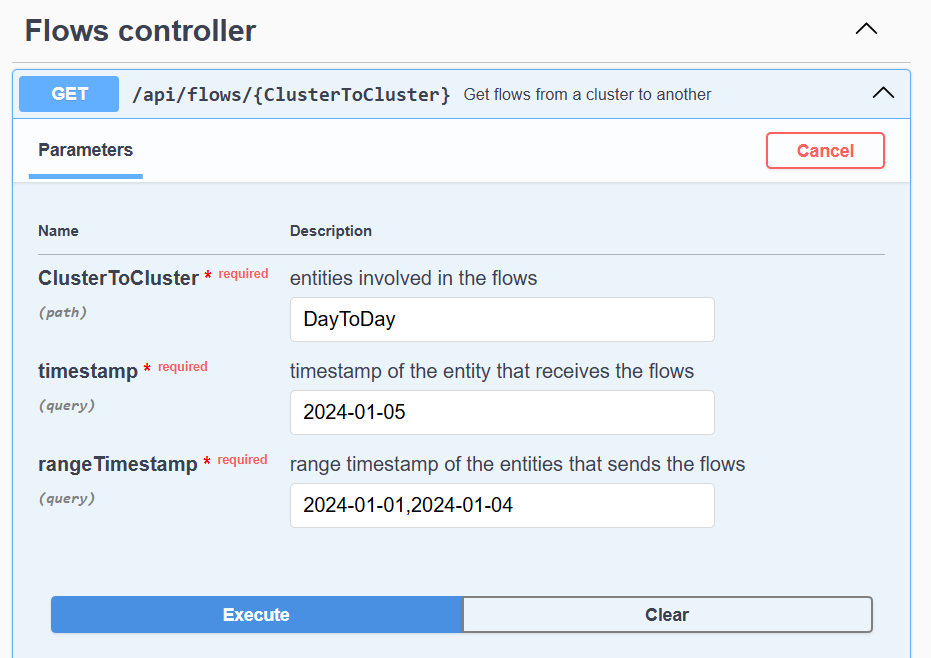
\includegraphics[keepaspectratio=true,scale=0.5]{Images/FlowControllerTestSwagger.png}
    \caption{Schermata Flow Controller della documentazione}
\end{figure}

In questo caso vengono richiesti i flussi tra Day-Cluster, il cui punto di partenza è definito dalle entità il cui timestamp è compreso nell'arco temporale che va dal 2024-01-01 al giorno 2024-01-04, mentre il punto di arrivo è il cluster con timestamp 2024-01-05.

\begin{figure}[H]
    \centering 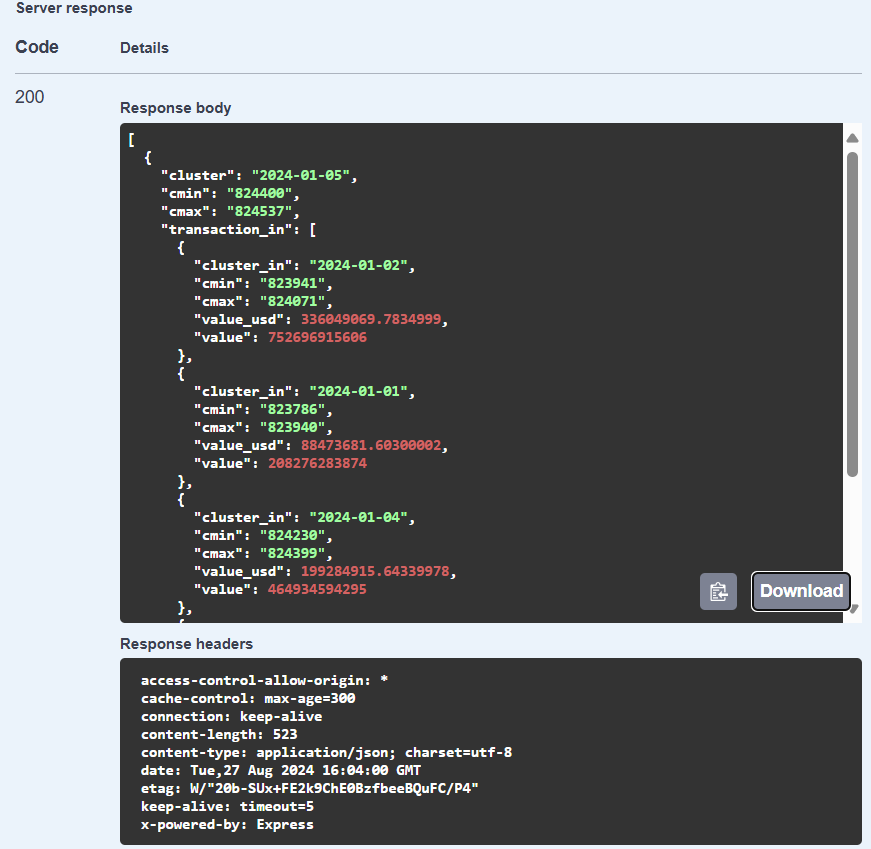
\includegraphics[keepaspectratio=true,scale=0.5]{Images/responseFlowController.png}
    \caption{Risposta della query effettuata tramite Flow Controller}
\end{figure}
In figura 21 viene mostrata la risposta inoltrata dal server per la gestione della richiesta effettuata tramite la sezione Flow Controller della documentazione.
La struttura generata per il JSON è in linea con quelle utilizzate per le visualizzazioni di BITVAS.
Ogni elemento dell'array corrisponde ai cluster di arrivo dei flussi considerati, che in questo caso è solo quello definito dal parametro timestamp, ovvero 2024-01-05.
L'array transaction$\_$in viene utilizzato per interpretare e rappresentare i flussi, infatti al suo interno vengono immagazzinati i Day-Cluster di partenza di questi ultimi, con relativo volume di cryptovaluta speso. 
\thispagestyle{mystyle}
\begin{figure}[H]
    \centering 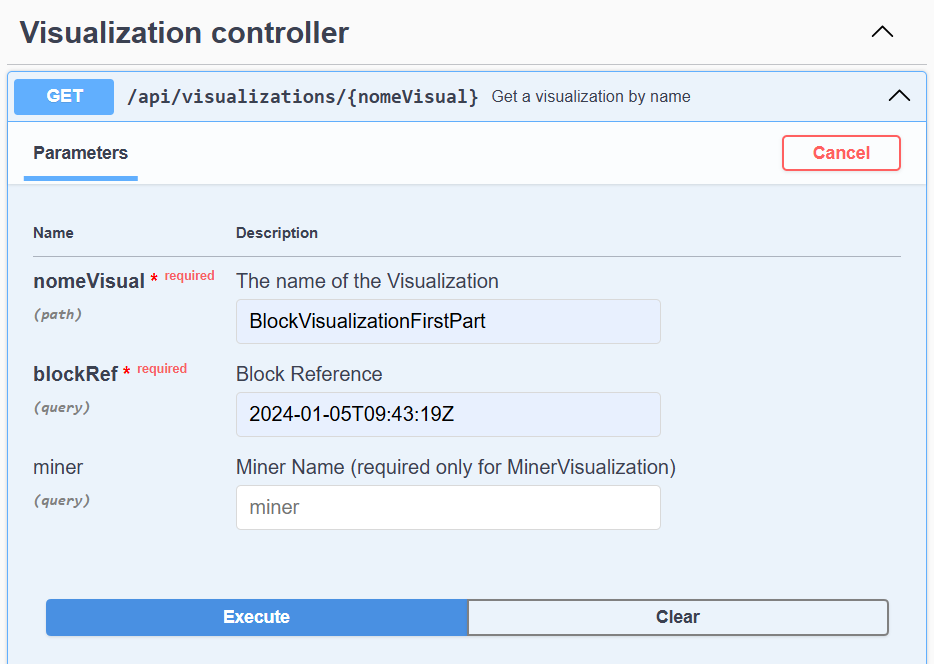
\includegraphics[keepaspectratio=true,scale=0.5]{Images/VisControllerSwaggerTest.png}
    \caption{Schermata Visualization Controller della documentazione}
\end{figure}
In questo caso, i parametri inseriti in input riguardano il nome della visualizzazione che si vuole ottenere, ovvero la prima parte della BlockVisualization e il timestamp di riferimento del blocco centrale di essa.
I risultati ottenuti e visualizzati di seguito, seguono la struttura dei file JSON già trattati in precedenza.
Per l'elemento che rappresenta il blocco centrale viene inizializzato un array, al cui interno vengono inseriti gli attributi riguardanti i blocchi da cui partono i flussi di Bitcoin.

La risposta fornita dal server fornisce solamente la prima parte della BlockVisualization, la quale si focalizza sui flussi in ingresso al blocco centrale.
Unendo quest'ultima con la risposta derivata dalla richiesta della seconda parte, si ottiene la risposta completa da integrare con BITVAS.

La scelta di effettuare una divisione della richiesta è dovuta alla possibilità di riutilizzo di tali dati in maniera diversa da quella definita dal tool di visualizzazione preso in esame.Questo approccio modulare consente una maggiore flessibilità nell’analisi dei dati, permettendo di eseguire query specifiche e di ottenere risposte mirate per diverse esigenze analitiche. Inoltre, facilita l’aggiornamento e la manutenzione del sistema, poiché ogni parte della visualizzazione può essere gestita e ottimizzata separatamente.
\thispagestyle{mystyle}
\begin{figure}[H]
    \centering 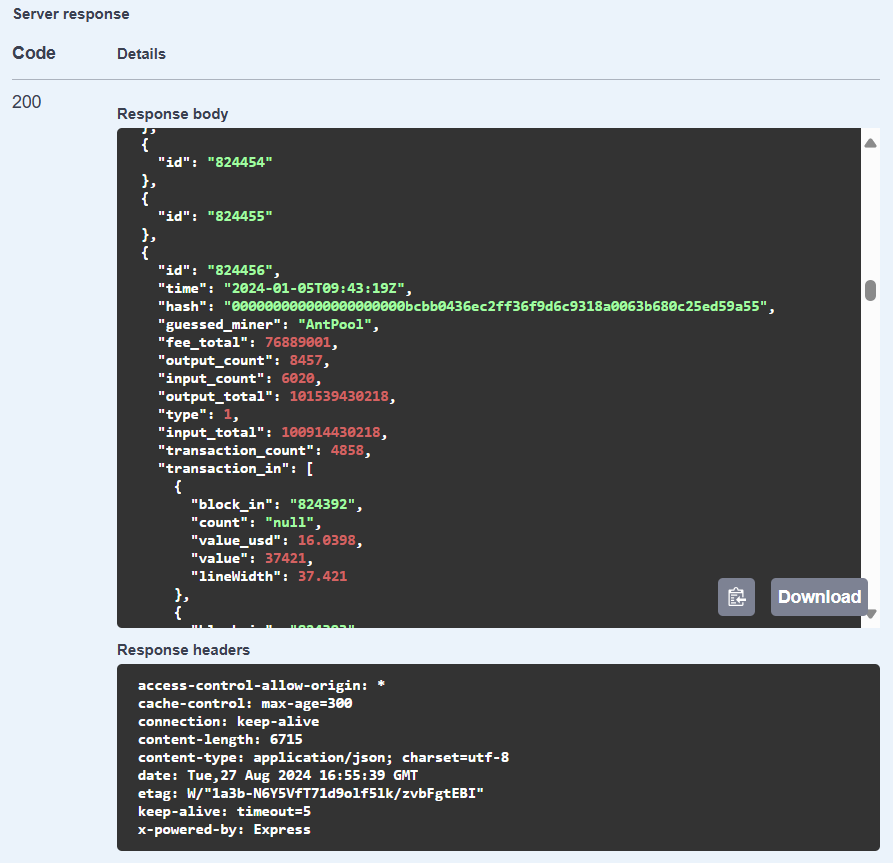
\includegraphics[keepaspectratio=true,scale=0.45]{Images/responseVisController.png}
    \caption{Risposta della query effettuata tramite Flow Controller}
\end{figure}


\begin{figure}[H]
    \centering 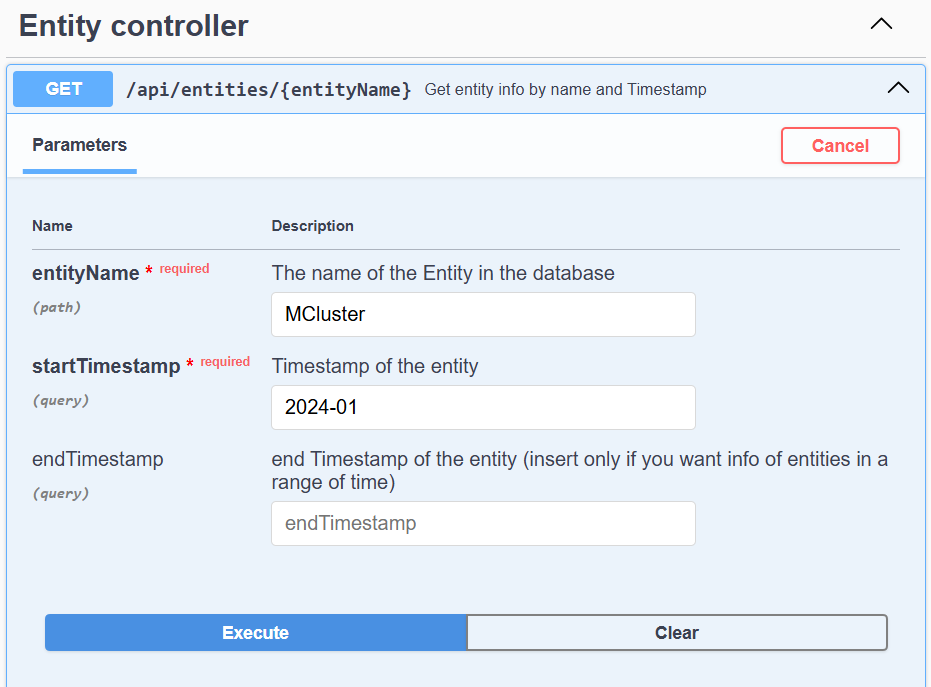
\includegraphics[keepaspectratio=true,scale=0.4]{Images/EntityControllerSwaggerTest.png}
    \caption{Schermata Entity Controller della documentazione}
    
    \thispagestyle{mystyle}
\end{figure}

In figura 24 viene mostrata la richiesta per le informazioni riguardanti un determinato Month-Cluster, identificato dal timestamp 2024-01.
\begin{figure}[H]
    \centering 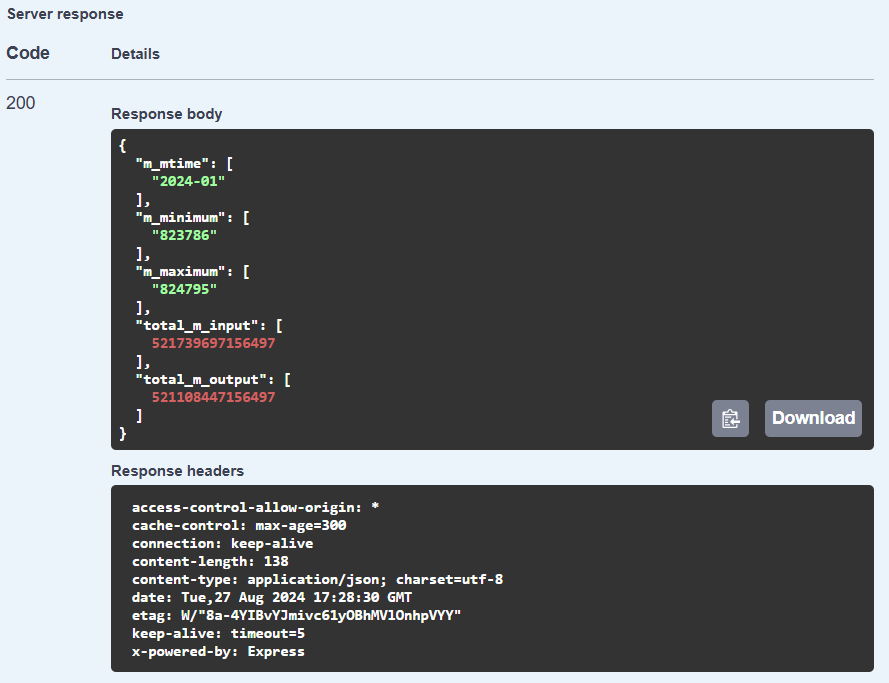
\includegraphics[keepaspectratio=true,scale=0.6]{Images/responseEntityController.png}
    \caption{Risposta della query effettuata tramite Entity Controller}
\end{figure}

La risposta fornita dal server è un file JSON i cui elementi sono degli array, ognuno dei quali corrisponde ad un attributo delle entità esratte, tra cui anche l'id minimo e massimo dei blocchi a cui essa fa riferimento.
In questo caso sono state richieste le informazioni di un solo MCluster, quindi è presente un solo elemento per ogni attributo.
\thispagestyle{mystyle}
Inoltre come per le risposte visualizzate precedentemente insieme alla risposta viene restituito un header con alcuni parametri fondamentali tra cui quelli utilizzati per la gestione del caching o il tipo contenuto in essa.

\subsection{Test di integrazione con BITVAS}
In questa sezione vengono mostrati i test effettuati per verificare il corretto reperimento dei dati necessari alle visualizzazioni di BITVAS.

L'API strutturata permette l'utilizzo del database a grafo ad applicativi esterni tramite la classe Request$\_$Controller, che mette a disposizione dei metodi per effettuare delle richieste GET al server.
Quest'ultima è stata integrata nel codice sorgente di BITVAS, in modo tale da rendere dinamico il reperimento dei dati.


\begin{figure}[H]
    \centering 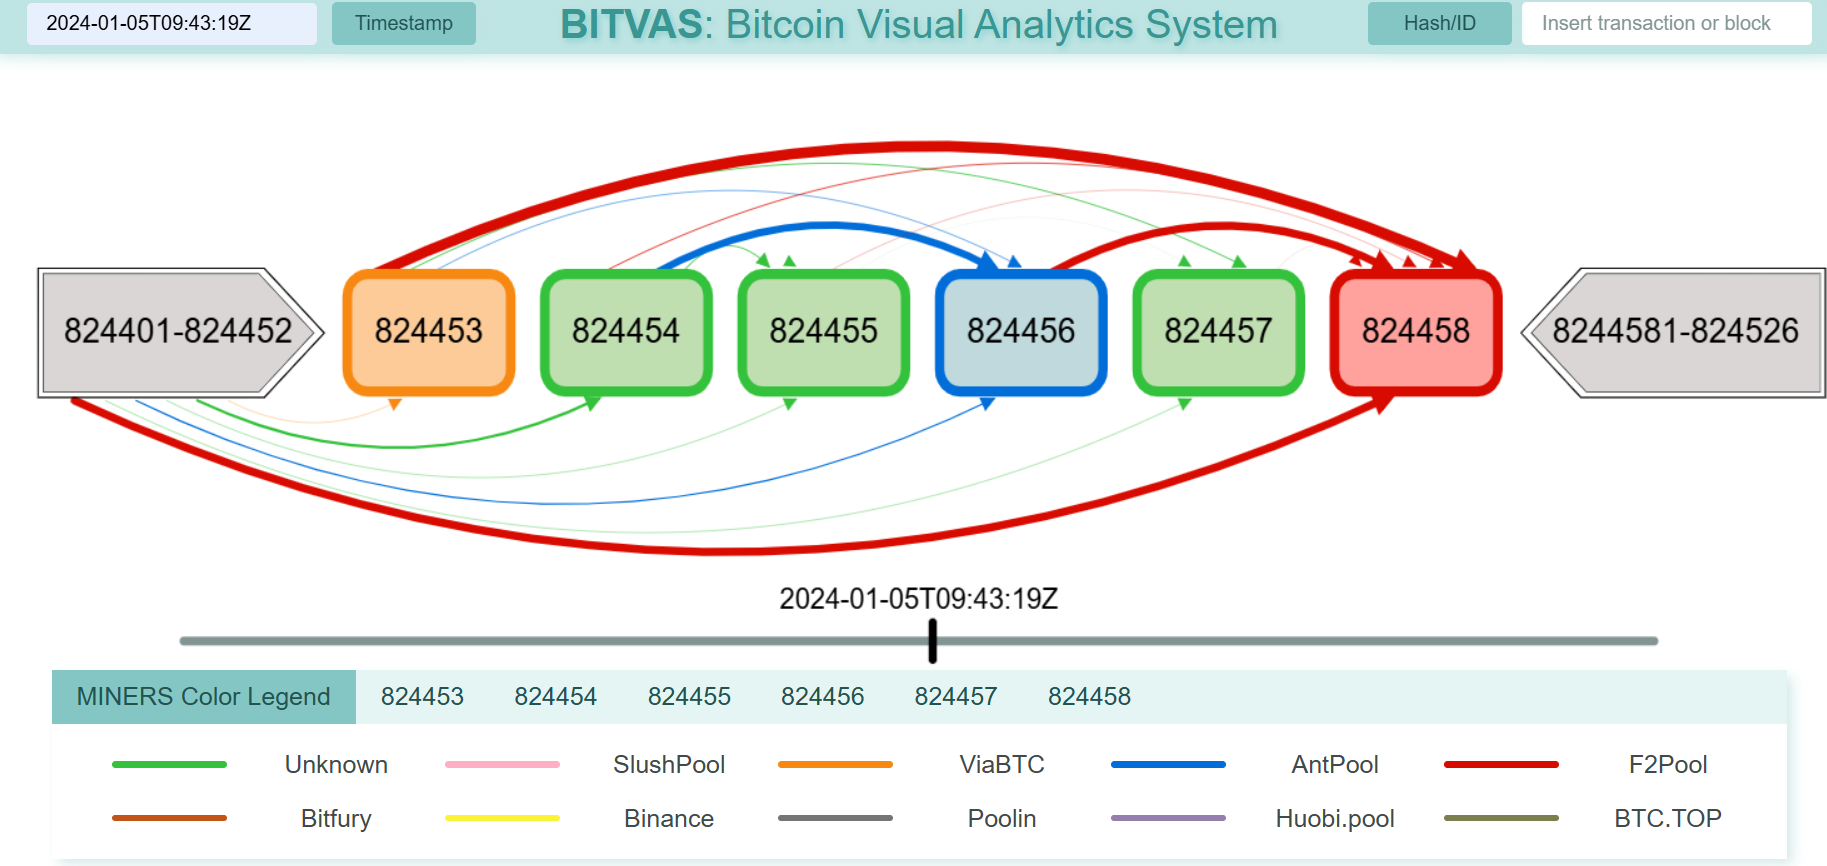
\includegraphics[keepaspectratio=true,scale=0.3]{Images/CombinedVisTested.png}
    \caption{Test CombinedVisualization}
\end{figure}

In figura 26 viene mostrata la visualizzazione dopo l'inserimento del timestamp '2024-01-05T09:43:19Z' in alto a sinistra, il cui blocco identificato da esso viene generato al centro della visualizzazione (824456).
Quest'ultimo si può modificare con lo slider posto al di sotto dei blocchi, traslando la visualizzazione blocco per blocco. 
Come ultimo elemento della schermata è presente una legenda interattiva con la quale richiedere la minerVisualization.
Nel caso del test effetuato viene scelto il miner 'AntPool', la cui visualizzazione viene mostrata di seguito.

\begin{figure}[H]
        \centering 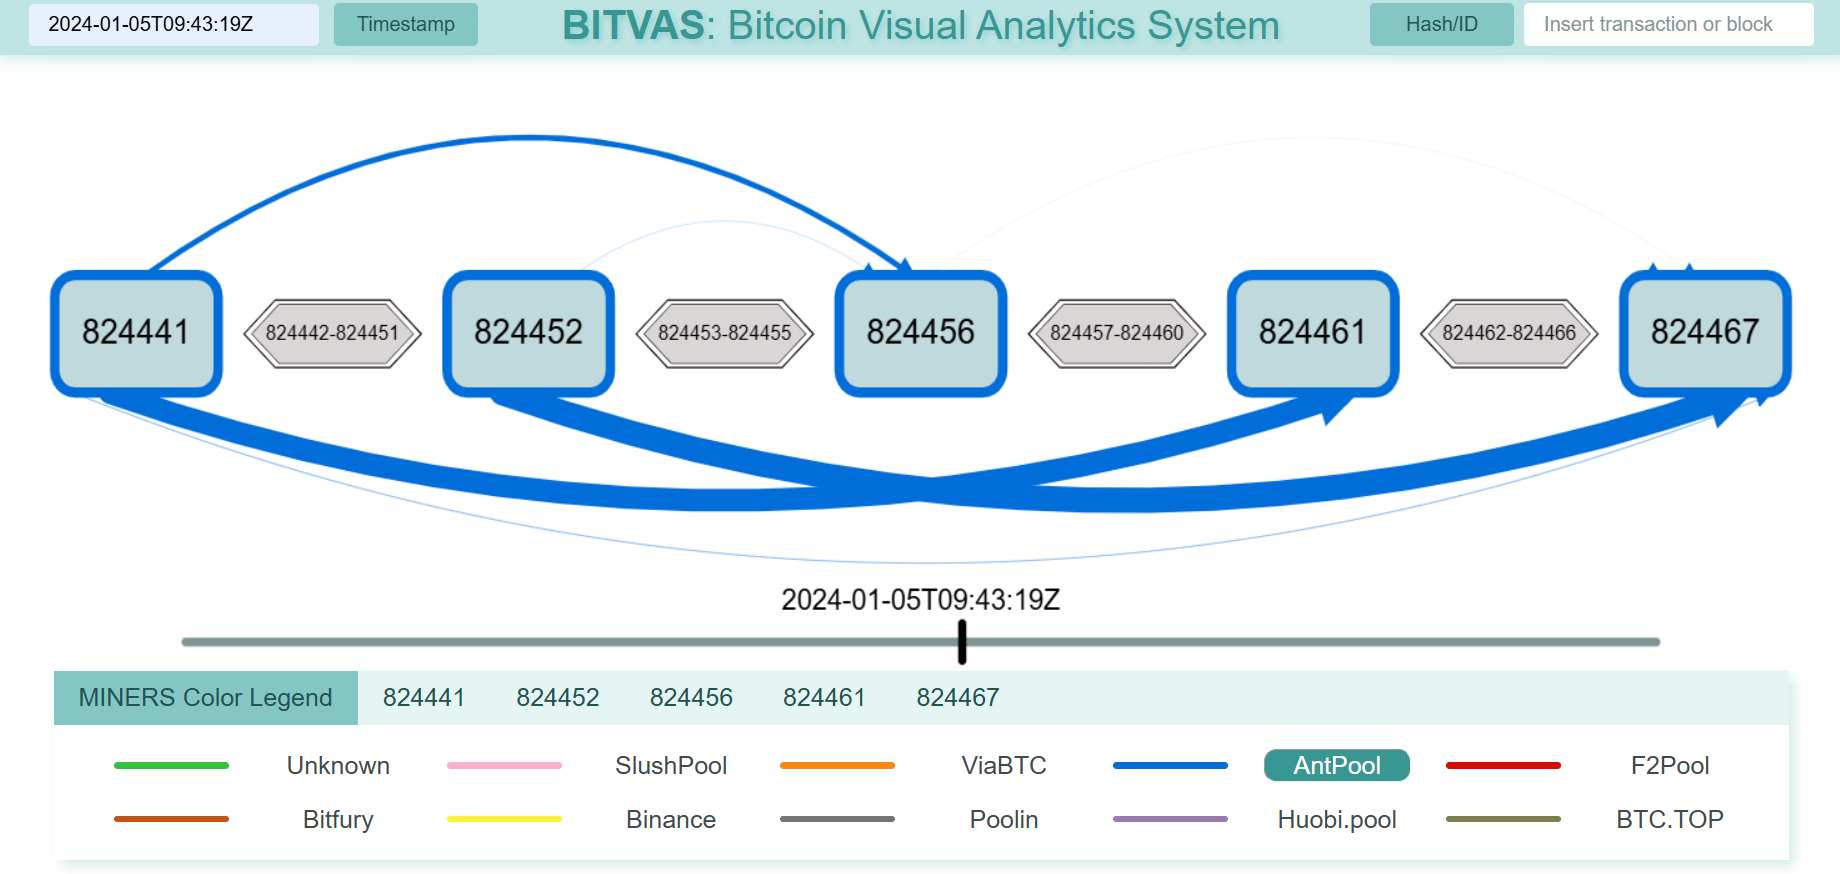
\includegraphics[keepaspectratio=true,scale=0.28]{Images/MinerVisualizationTest.png}
    \caption{Test MinerVisualization}
\end{figure}
\thispagestyle{mystyle}
Anche in questo caso il blocco identificato dalla posizione dello slider, ovvero quello inserito come input per la visualizzazione iniziale, si trova al centro di essa.
Nel caso in cui il blocco scelto non faccia parte dei flussi legati al miner selezionato, tramite i moduli di creazione dei JSON viene scelto come blocco centrale quello il cui timestamp è più vicino ad esso temporalmente.

\thispagestyle{mystyle}

